%macbook 
\begin{vidu}
Trên mặt hồ yên lặng, một người làm cho con thuyền nhỏ dao động tạo ra sóng trên mặt nước. Thuyền thực hiện được 24 dao động trong $40\ s$, mỗi dao động tạo ra một ngọn sóng cao $12\ cm$ so với mặt hồ nước yên lặng và ngọn sóng tới bờ cách thuyền $10\ m$ sau $5\ s$. Bỏ qua sự tắt dần của sóng.
\begin{itemize}
\item[1,] Chu kì dao động của thuyền là .............
\item[2.] Tốc độ lan truyền của sóng là ..........
\item[3.] Bước sóng là .............
\item[4.] Biên độ sóng là .............
\end{itemize}
\loigiai{
\begin{itemize}
\item[1.] Chu kì dao động của thuyền là: $T=\dfrac{\Delta t}{N}=\dfrac{40}{24}=\dfrac{5}{3}\ s$.
\item[2.] Tốc độ lan truyền của sóng là: $v=\dfrac{s}{t}=\dfrac{10}{5}=2\ m/s$.
\item[3.] Bước sóng là:  $\lambda=v.T=2.\dfrac{5}{3}=\dfrac{10}{3}\ m$.
\item[4.] Biên độ sóng là: $A=12\ cm$.

\end{itemize}
}
\end{vidu} \haidong{20}
\begin{vidu}%KNTT
Một sóng âm có tần số $192\ Hz$ và truyền đi được quãng đường $91,4\ m$ trong $0,27\ s$.
\begin{itemize}
\item[1.] Tốc độ truyền sóng là ..........
\item[2.] Bước sóng  là ..........
\item[3.] Nếu tần số sóng là 442 Hz thì bước sóng  là .......... và chu kì là ..........
\end{itemize}
\loigiai{
\begin{itemize}
\item[1.] $v=\dfrac{s}{t}=\dfrac{91,4}{0,27}=338,5\ m/s$.
\item[2.] $v=\lambda f\Rightarrow \lambda=\dfrac{v}{f}=\dfrac{338,5}{192}=1,76\ m$
\item[3.] $\lambda'=\dfrac{v}{f'}=\dfrac{338,5}{442}=0,77\ m;\ T'=\dfrac{1}{f'}=\dfrac{1}{442}=0,002\ s$
\end{itemize}
}
\end{vidu} \haidong{20}


\loai{Thay số tính bước sóng}
\begin{vidu}%[3P2-1.2Y][Loai1]
Một sóng cơ truyền trên một sợi dây rất dài với tốc độ 1 m/s và chu kì 0,5 s. Sóng cơ này có bước sóng là
\choice
{25 cm}
{100 cm}
{\True 50 cm}
{150 cm}
\loigiai{
Bước sóng: $\lambda =v. T=100. 0,5=50\ cm$.
}
\end{vidu} \haidong{20}
\loai{Thay số tính tần số}
\begin{vidu}%[3P2-1.2B][Loai1]  
Một sóng truyền trong một môi trường với vận tốc 110  m/s và có bước sóng 0,25 m. Tần số của sóng này là 
\choice
{\True 440 Hz}
{220 Hz}
{110 Hz}
{660 Hz}
\loigiai{
Tần số của sóng: $f=\dfrac{v}{\lambda}=\dfrac{110}{0,25}=440\ Hz$.
}
\end{vidu} \haidong{20}
\loai{Quãng đường lan truyền của sóng}
\begin{vidu}%[3P2-1.2B][Loai1]
Một sóng cơ có chu kì 1,8 s truyền trên sợi dây rất dài. Sau 4 s chuyển động truyền được 20 m dọc theo dây. Bước sóng của sóng tạo thành trên dây
\choice
{\True 9 m}
{6 m}
{4 m}
{3 m}
\loigiai{
\begin{itemize}
\item Tốc độ truyền sóng là $v = \dfrac{20}{4} = 5$ m/s.
\item Bước sóng là $\lambda  = v. T = 9$ m.
\end{itemize}
}
\end{vidu} \haidong{20}
\loai{Quan sát phao nhô lên}
\begin{vidu}%[3P2-1.2B][Loai1]
Một người quan sát trên mặt nước biển thấy một cái phao nhô lên 5 lần trong 20 s và khoảng cách giữa hai đỉnh sóng liên tiếp là 2 m. Tốc độ truyền sóng biển là
\choice
{\True 40 cm/s}
{50 cm/s}
{60 cm/s}
{80 cm/s}
\loigiai{
\begin{itemize}
\item Hai ngọn sóng liên tiếp cách nhau $\lambda  = 2$ m.
\item  Khoảng thời gian quan sát phao nhô lên cao 5 lần là 4 chu kì $\Rightarrow  T = \dfrac{20}{4} = 5\ s\Rightarrow  v = \dfrac{\lambda}{T} = 40$ cm/s.
\end{itemize}
}
\end{vidu} \haidong{20}
\loai{Sóng lan truyền trong các môi trường}
\begin{vidu}%[3P2-1.2B][Loai1]
Tốc độ âm trong nước là 1530 m/s, trong không khí là 340 m/s. Khi âm truyền từ không khí vào nước, bước sóng của nó
\choice
{không đổi}
{\True tăng 4,5 lần}
{giảm 4,5 lần}
{giảm 1190 lần}
\loigiai{
Ta có: $\dfrac{\lambda_{H_2O}}{\lambda_{kk}}=\dfrac{v_{H_2O}}{v_{kk}}=4,5$. 
}
\end{vidu} \haidong{20}
\loai{Tốc độ truyền sóng - tốc độ dao động}
\begin{vidu} %[3P2-1.2K][Loai1]
Một sóng cơ học có biên độ không đổi A, bước sóng $\lambda$. Vận tốc dao động cực đại của phần tử môi trường bằng 4 lần tốc độ truyền sóng khi
\choice
{$\lambda =\pi A$}
{$\lambda =2\pi A$}
{\True $\lambda =\dfrac{\pi A}{2}$}
{$\lambda =\dfrac{\pi A}{4}$}
\loigiai{
\begin{itemize}
\item Ta có: $v_{\max}=4v_s\Rightarrow \omega A=4\dfrac{\lambda}{T}\Rightarrow \dfrac{2\pi}{T}A=4\dfrac{\lambda}{T}\Rightarrow \lambda =0,5\pi A$. 
\end{itemize}
}
\end{vidu} \haidong{20}
\loai{Quãng đường truyền sóng - quãng đường dao động}
\begin{vidu}%[3P2-1.2K][Loai1]  
Một sóng cơ lan truyền trong một môi trường với tốc độ 1 m/s và tần số 10 Hz, biên độ sóng không đổi là 4 cm. Khi phần tử vật chất nhất định của môi trường đi được quãng đường S thì sóng truyền thêm được quãng đường 25 cm. Giá trị S bằng
\choice
{24 cm}
{25 cm}
{56 cm}
{\True 40 cm}
\loigiai{
\begin{itemize}
\item Ta có: $T=\dfrac{1}{f}=\dfrac{1}{10}=0,1\ s\Rightarrow \dfrac{T}{2}=0,05\ s$.
\item Quãng đường truyền sóng: $\Delta S=v.\Delta t\Rightarrow \Delta t=\dfrac{\Delta S}{v}=\dfrac{0,25}{1}=0,25\ s=5.\dfrac{T}{2}$.
\item Quãng đường dao động: $S=5.2A=5.2.4=40\ cm$.
\end{itemize}
\textbf{Chú ý:} Phân biệt tốc độ truyền sóng và tốc độ dao động cực đại:
$\begin{cases}
v_s=\dfrac{\lambda}{T}\\
v_{\max}=\omega A=\dfrac{2\pi}{T}A\\
\end{cases}\Rightarrow \dfrac{v_{\max}}{v_s}=\dfrac{2\pi A}{\lambda}$.
}
\end{vidu} \haidong{20}











%macbook 

\begin{vidu}
\immini[thm]{
Hình bên là đồ thị $(u-t)$ của một sóng âm trên màn hình của một dao động kí. Biết mỗi cạnh của ô vuông theo phương ngang trên hình tương ứng với 1 ms. Tần số của sóng là
\choice
{3 Hs}
{$\dfrac{1}{3}$ Hz}
{\True $\dfrac{1000}{3}$ Hz}
{$\dfrac{3}{1000}$ Hz}
}{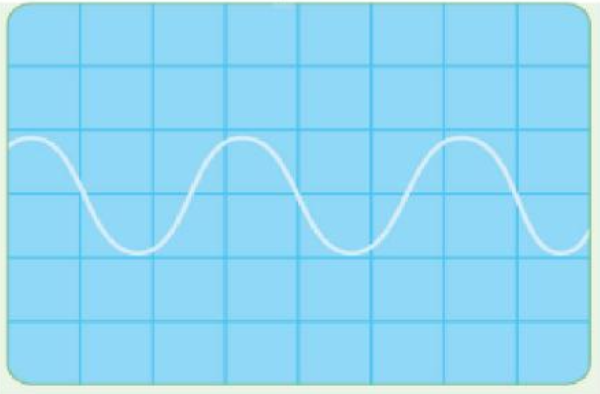
\includegraphics[width=4cm]{Hinh/KN84}}
\loigiai{
\begin{itemize}
\item Chu kì sóng: $T=3\ ms=3.10^{-3}\ s$. 
\item Tần số sóng: $f=\dfrac{1}{T}=\dfrac{1000}{3}\ Hz$. 
\end{itemize}
}
\end{vidu} \haidong{20}
\loai{Sự truyền âm}
\begin{vidu}%[3P2-11.2K][Loai1]
Sóng âm khi truyền trong chất rắn có thể là sóng dọc hoặc sóng ngang và lan truyền với tốc độ khác nhau. Tại trung tâm phòng chống thiên tai nhận được hai tín hiệu sóng từ một vụ động đất cách nhau một khoảng thời gian 240 s. Biết tốc độ truyền sóng ngang và tốc độ truyền sóng dọc trong lòng đất có giá trị lần lượt là 5 km/s và 8 km/s. Tâm chấn động cách nơi nhận tín hiệu một khoảng 
\choice
{\True 3200 km}
{570 km}
{730 km}
{3500 km}
\loigiai{
\begin{itemize}
\item Gọi d là khoảng cách từ tâm chấn động đến nơi nhận tín hiệu, ta có:
$\dfrac{d}{5}-\dfrac{d}{8}=240\Rightarrow d=3200$ km. 
\end{itemize}
}
\end{vidu} \haidong{20}
\begin{vidu}%[3P2-11.2K][Loai1]
Để ước lượng độ sâu của một giếng cạn nước, một người dùng đồng hồ bấm giây, ghé sát tai vào miệng giếng và thả một hòn đá rơi tự do từ miệng giếng, sau 3 s thì người đó nghe thấy tiếng hòn đá đập vào đáy giếng. Giả sử tốc độ truyền âm trong không khí là $330\ m/s$, lấy $g = 9,9\ m/s^2$. Độ sâu ước lượng của giếng là
\choice
{39 m}
{43 m}
{\True 41 m}
{45 m}
\loigiai{
\begin{itemize}
\item Độ sâu của giếng: $h = \dfrac{9. 9t_1^{2}}{2}=330(3-t_1)\Rightarrow t_1\Rightarrow h\approx 41\ m$.  
\end{itemize}
}
\end{vidu} \haidong{20}














%macbook 
\loai{Tỉ lệ I và r}
\begin{vidu}%CTST
\immini[thm]{
Một còi báo động có kích thước nhỏ phát sóng âm trong môi trường đồng chất, đẳng hướng. Ở vị trí cách còi một đoạn 15 m, cường độ sóng âm là $0,25\ W/m^2$. Vậy ở khoảng cách nào từ vị trí của còi thì sóng âm có cường độ bằng $0,01\ W/m^2$?
\motcot
{65 m}
{\True 75 m}
{85 m}
{95 m}
}{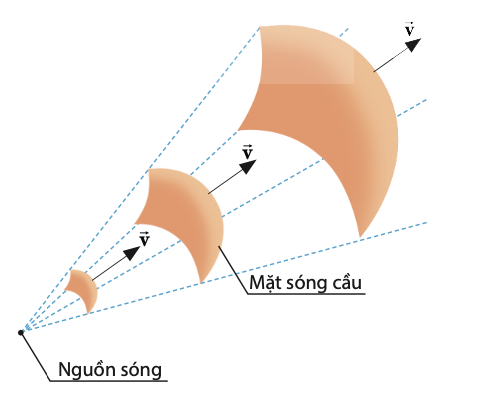
\includegraphics[width=4cm]{Hinh/CT68}}
\loigiai{
\begin{itemize}
\item Vì nguồn âm được xem như một điểm nên sóng âm có mặt sóng là mặt cầu có diện tích $S=4\pi r^2$, với r là bán kính mặt cầu (cũng là khoảng cách từ điểm đang xét đến còi).
\item Tại vị trí $r_1=15\ m$ và $r_2$, ta có: $I_1=\dfrac{P}{4\pi r_1^2}$ và $I_2=\dfrac{P}{4\pi r_2^2}$
\item Suy ra: $\dfrac{I_1}{I_2}=\dfrac{r_2^2}{r_1^2};\ r_2=r_1\sqrt{\dfrac{I_1}{I_2}}=15\sqrt{\dfrac{0,25}{0,01}}=75\ m$.
\item Vậy ở khoảng cách 75 m tính từ vị trí của còi thì sóng âm có cường độ bằng $0,01\ W/m^2$.
\end{itemize}
}
\end{vidu} \haidong{20}
\loai{Tỉ lệ P và r}
\begin{vidu}%[3P2-11.3K][Loai1]}
Một nguồn điểm phát âm đẳng hướng trong môi trường không hấp thụ âm. Công suất của nguồn phát không đổi. Tiến hành đo độ to của âm tại một điểm cách nguồn 16 m. Sau đó giảm công suất nguồn âm xuống còn một nửa. Muốn đo được độ to của âm như cũ thì phải di chuyển tới vị trí cách nguồn âm một khoảng bằng
\choice
{$8\ m$}
{$\dfrac{8}{\sqrt2}\ m$}
{$16\sqrt2\ m$}
{\True $8\sqrt2\ m$}
\loigiai{
\begin{itemize}
\item Ta có: $I = \dfrac{P}{4\pi r^2} = I_0.10^L$
\item Sau khi giảm công suất một nửa thì $I' = \dfrac{P}{2.4\pi r'^2}$
\item Do độ to như cũ nên $I=I'$: $\dfrac{1}{r^2} = \dfrac{1}{2r'^2} \Rightarrow r' = \dfrac{r}{\sqrt{2}} = 8\sqrt{2}$ m. 
\end{itemize}
}
\end{vidu} \haidong{20}
\begin{vidu}%[3P2-12.2K][Loai1]  
\immini[thm]{Hai nguồn âm điểm phát sóng âm phân bố đều theo mọi hướng, bỏ qua sự hấp thụ và phản xạ âm của môi trường. Hình vẽ bên là đồ thị phụ thuộc cường độ âm I theo khoảng cách đến nguồn r (nguồn 1 là đường 1, nguồn 2 là đường 2). Tỉ số công suất nguồn 1 và công suất nguồn 2 là
\choice
{0,25}
{\True 2}
{4}
{0,5}}{\begin{tikzpicture}[scale=1,thick,>=stealth',x=0.4cm,y=0.4cm]
\tkzDefPoints{0/0/o, 12/0/x, 0/7/i}
\draw[red,very thick] plot [smooth,tension=1] coordinates{(0.5,6)(3.5,2) (11,0.6)};
\draw[blue,very thick] plot [smooth,tension=1] coordinates{(0.5,3.5)(3.5,1) (11,0.3)};
\foreach  \y  in  {1,2,3,4}
{\draw[dashed, thin]  (0,\y)  -- (11,\y);}
\tkzDrawSegments[->](o,x o,i)
\node at (x)[below]{$r\ (m)$};
\node at (i)[right]{$I\ (W/m^2)$};
\node at (0.5,5.5)[right]{$(1)$};
\node at (2,1.5)[below]{$(2)$};
\node at (o)[below left]{$O$};
\draw[thin,dashed](3.5,4)--(3.5,0)node[below]{$1$};
\end{tikzpicture}}
\loigiai{
\begin{itemize}
\item Tại cùng một vị trí r thì $I_1 = 2I_2 \Rightarrow  P_1 = 2P_2$. 
\end{itemize}
}
\end{vidu} \haidong{20}


